% 泰勒展开
% 微积分|导数|高阶导数|泰勒展开|泰勒级数

\pentry{高阶导数\upref{HigDer}}

若一个函数在某个区间内可以求任意阶的导数(例如幂函数,三角函数,指数函数,对数函数等),那么这个函数可以用一个多项式近似,且总项数 $N$ 越多,近似得越精确. 令多项式为
\begin{equation}\label{Taylor_eq1}
f(x) \approx c_0 + c_1(x - x_0) + c_2(x - x_0)^2 +  \ldots  = \sum_{n = 0}^N  c_n (x - x_0)^n
\end{equation}
其中 $x_0$ 是该区间内的任意一点,多项式每一项的系数由函数在 $x_0$ 处的第 $n$ 阶导数求得
\begin{equation}\label{Taylor_eq2}
c_n = \frac{1}{n!} f^{(n)}(x_0)
\end{equation}
注意其中 0 的阶乘为 $0! = 1$. 另外由\autoref{Taylor_eq1} 得,当 $x=x_0$ 时,函数值等于多项式值. 当项数 $N$ 有限时,通常 $\abs{x-x_0}$ 越小多项式就越接近函数 . 以上这种把函数展开成多项式的方法就叫\textbf{泰勒展开}. 我们先来看一个例子

\begin{example}{正弦函数}
我们在 $x_0=0$ 处展开 $\sin x$, 由\autoref{Taylor_eq1} 和\autoref{Taylor_eq2} 得
\begin{equation}\label{Taylor_eq3}
\sin x = x - \frac{1}{3!}{x^3} + \frac{1}{5!}{x^5} - \frac{1}{7!} x^7 + \ldots 
\end{equation}
取不同的项数 $N$ 求和,画图如\autoref{Taylor_fig1}. 可见随着项数增加,多项式慢慢趋近正弦函数.

\begin{figure}[ht]
\centering
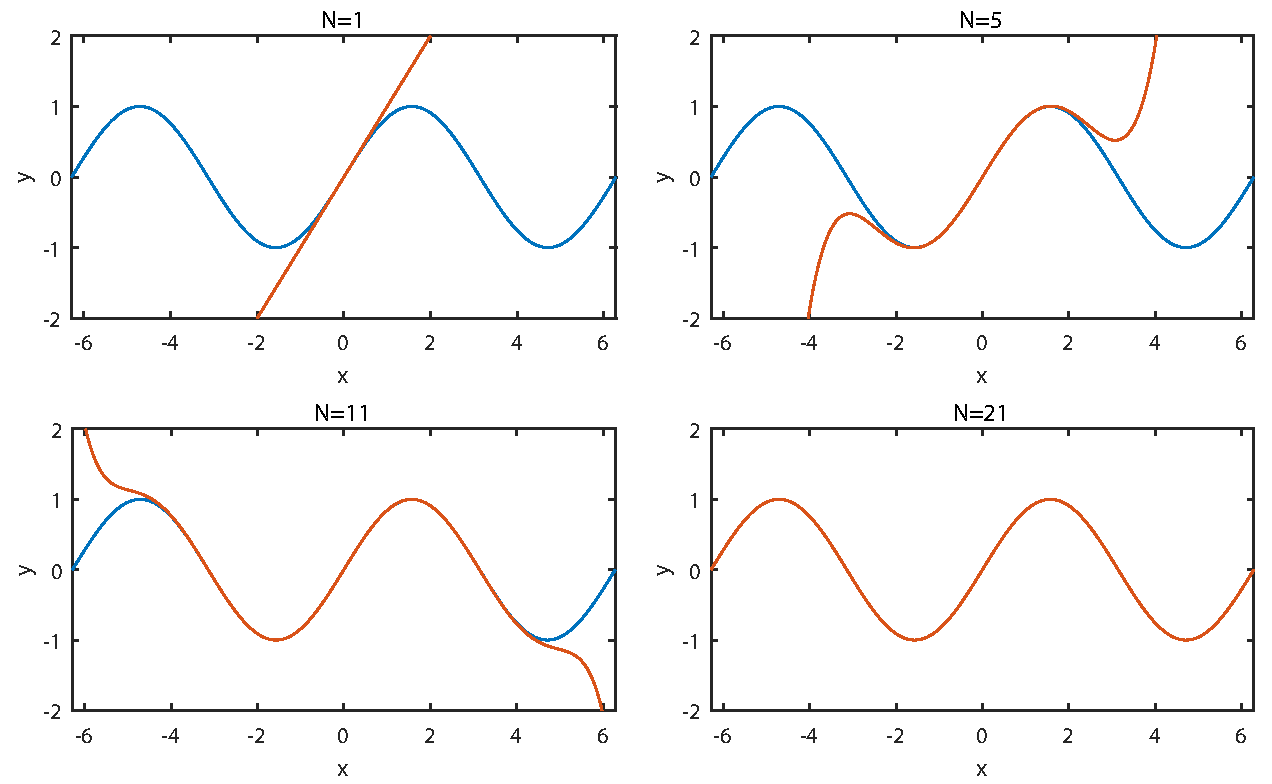
\includegraphics[width=14cm]{./figures/Taylor_1.pdf}
\caption{$\sin x$ 在原点处的泰勒展开的前 $N$ 项求和.容易看出,求和的项数越多,多项式(橙)与 $\sin x$ (蓝)吻合得越好.}\label{Taylor_fig1}
\end{figure}
\end{example}

\subsection{系数公式的推导}
我们假设当项数 $N \to \infty$ 时, 存在唯一的多项式在某区间内处处趋于无穷可导函数\footnote{这叫做多项式的完备性,这里不作证明.} $f(x)$,即
\begin{equation}\label{Taylor_eq5}
f(x) = \sum_{n = 0}^\infty  c_n (x - x_0)^n
\end{equation}
首先代入 $x = x_0$,可得第一个系数 $c_0 = f(x_0)$. 现在我们对上式两边在 $x_0$ 处求导,得
\begin{equation}
f'(x_0) = c_1 + \eval{ \sum_{n = 2}^\infty n c_n (x - x_0)^{n - 1} }_{x = x_0}  = c_1
\end{equation}
如果对\autoref{Taylor_eq5} 两边在 $x_0$ 处求二阶导数,得
\begin{equation}
f''(x_0) = 2 c_2 + \eval{ \sum_{n = 3}^\infty  n(n - 1) c_n (x - x_0)^{n - 2} }_{x = x_0}  = 2 c_2
\end{equation}
即 $c_2 = f''(x_0)/2!$.  以此类推,如果对\autoref{Taylor_eq5} 两边在 $x_0$ 处求 $m$ 阶导数得
\begin{equation}
f^{(m)}(x_0) = m! c_m + \eval{ \sum_{n = m + 1}^\infty  \frac{n!}{(n - m)!} c_n (x - x_0)^{n - m} }_{x = x_0}  = m! c_m
\end{equation}
所以系数公式为
\begin{equation}
{c_m} = \frac{1}{m!} f^{(m)}(x_0)
\end{equation}

泰勒展开的存在说明了无穷可导函数的一个重要性质:任何一点的性质都能决定完整的函数曲线,这可以类比生物中用一个细胞克隆出一个完整生物体.

\subsection{一些常见函数关于原点的泰勒展开}
作为练习,请验证以下泰勒展开式

\begin{equation}
\sin x = x - \frac{1}{3!} x^3 + \frac{1}{5!} x^5 - \frac{1}{7!} x^7 \ldots
\end{equation}
\begin{equation}
\cos x = 1 - \frac{1}{2!} x^2 + \frac{1}{4!} x^4 -\frac{1}{6!} x^6 \ldots
\end{equation}
\begin{equation}\label{Taylor_eq11}
\E^x =1 + x + \frac{1}{2!} x^2 + \frac{1}{3!} x^3  \ldots
\end{equation}
\begin{equation}
\ln (1+x) = x - \frac12 x^2 + \frac13 x^3 - \frac14 x^4 \ldots
\end{equation}
\begin{equation}
\frac{1}{1+x} = 1 - x + x^2 - x^3 \ldots
\end{equation}
\begin{equation}
\sqrt{1+x} = 1 + \frac12 x - \frac18 x^2 + \frac{1}{16} x^3 \ldots
\end{equation}

\subsection{泰勒展开与近似}
事实上,泰勒展开可以看成是微分近似\upref{Diff}的一种高阶拓展. 微分近似中,在某点 $x_0$ 附近有
\begin{equation}
f(x) \approx f(x_0) + f'(x_0)(x - x_0)
\end{equation}
而这恰好是泰勒展开的前两项. 然而,这只是函数曲线在 $x_0$ 处的切线(见\autoref{Taylor_fig1} 中 $N=1$ 的情况),显然没有高阶的泰勒展开那么精确. 如果我们将 $f(x)$ 近似到其泰勒展开的 $x^n$ 项, 我们称这个近似精确到第 $n$ 阶, 因为它的误差小于或等于 $n + 1$ 阶无穷小\upref{Lim} $\order{x^{n + 1}}$.
